% !TeX root = ../thuthesis-example.tex

\chapter{Kernel-level optimizations}\label{chapter-6}
In this chapter we introduce the design and implementation of the two specialized GPU kernels in use by ExpertFlow. The first customized kernel is used to implement the fused-experts operator, which computes the predictions of a group of MoE experts assigned to the same device using a single kernel. The second customized kernel is used by the multi-head attention layers. While cuDNN already offers a heavily-optimized kernel for multi-head attention, it does not support caching the key and value projections, which is required for incremental decoding. In addition, it does not support the optimizations we require for speculative inference. In the following sections, we discuss the considerations that led us to the final version of each kernel, as well as the optimizations that we used. 

\section{Fused-Experts Operator}\label{section-fused-experts}
An essential factor to be able to run a Mixture-of-Experts model without incurring in great performance overhead is to use efficient GPU kernels. In particular, a MoE layer generally requires a fast implementation of a \textit{gating network}, \textit{top-k}, \textit{token dispatch}, \textit{expert prediction}, and \textit{predictions aggregation} kernel. In this section, we illustrate the role of each kernel, and how we implemented each of them in our \textit{fused-experts operator} in order to significantly optimize the performance when compared to the naive version.

\subsection{MoE-layer kernels}

\begin{algorithm}[H]
  \caption{Naive MoE-layer algorithm}
  \label{alg:naive-moe}
  \small
  \begin{algorithmic}[1]
    \Ensure $x$: input sequence, $W_{i}$: weights of expert $i \in [0, E)$, $GatingNetwork$: the weights of the FFN that implements the gating network, $k$: how many experts to route each token to, $E$: total number of experts, $C$: expert capacity, $seq\_len$: maximum number of tokens in each request, $batch\_size$: number of requests in each batch, $emb\_dim$: embedding dimension
    \Require shape of $x = [emb\_dim, seq\_len \cdot batch\_size]$
    \Require shape of $W_{i} = [emb\_dim, emb\_dim]$
    \Require $k \leq E$
    \State num\_tokens $\leftarrow$ seq\_len $\cdot$ batch\_size
    \State g $\leftarrow$ Softmax(GatingNetwork(x))
        \Comment{gating network kernel}
    \State top\_values, top\_indices $\leftarrow$ TopK(g)
        \Comment{top-k kernel}
    \State z $\leftarrow$ \Call{OneHotEncoding}{top\_indices, k, E, num\_tokens, C}
        \Comment{token dispatch kernel}
    \State predictions $\leftarrow$ x $\times$ z $\times \begin{bmatrix} W_0, \ \dots, \ W_{E-1} \end{bmatrix}^\top$
        \Comment{expert prediction kernel}
    \State output $\leftarrow$ dot(top\_values, predictions)
        \Comment{predictions aggregation kernel}
    \State 
    \Procedure{OneHotEncoding}{top\_indices, $k$, $E$, $num\_tokens$, $C$}
        \State Allocate a size of $k \cdot E \cdot num\_tokens $ for tensor $z$
        \State Allocate a size of $E$ for boolean array $num\_assignments$
        \State $z \leftarrow \{0\}$
        \State $num\_assignments \leftarrow \{0\}$
        \For{i}{0}{$num\_tokens$}
            \For{j}{0}{$k$}
                \State $e \leftarrow top\_indices[j,i]$
                \If{ $num\_assignments[e] \leq C$ }
                    \State $num\_assignments \leftarrow num\_assignments + 1$
                    \State $z[j,e,i] = 1$
                \EndIf
            \EndFor
        \EndFor
        \State return $z$
    \EndProcedure
  \end{algorithmic}
\end{algorithm}

Above, we present a naive algorithm (Algorithm \ref{alg:naive-moe}) to implement a MoE layer. In this version, we focus on the vanilla MoE model where each expert consists of a single fully-connected layer, and the gating network is also made up of a single fully-connected layer, followed by a softmax and a top-k. More realistic MoE layers will use more advanced components to achieve better load balancing, and improve the model's generalization power; for instance, several models~\cite{g-shard, original_moe}  add a stochastic components in the gating network. These additional components, however, are for the most part orthogonal to the issues we are discussing here, so we omit them for simplicity.

Each of lines 2-6 corresponds to one of the five typical MoE kernels introduced above. The algorithm should help demystifying what each such kernel does, and the dependencies between the kernels. We can implement Algorithm \ref{alg:naive-moe} in CUDA using a cuBLAS GEMM operator for the matrix multiplication steps, cuDNN for the softmax, and a custom CUDA kernel for the remaining steps. We can further implement a single fused kernel using CUDA or CUTLASS. However, the sparsity introduced by the one-hot encoding, together with the sequential nature of the two for loops (which are difficult to parallelize due to the need to consider the expert capacity when assigning tokens to experts) within the \textsc{OneHotEncoding} procedure lead the naive algorithm to suffer from poor performance in practice.

\subsection{ExpertFlow fast kernel implementation}
In ExpertFlow, we speed up the implement the \textit{token dispatch}, \textit{expert prediction}, and \textit{predictions aggregation} through the kernels shown below. In particular, Algorithm \ref{alg:moe-sort-tokens} allows us to parallelize the token dispatch operation, without exceeding the expert capacity. The kernel is carefully constructed so that each instruction is fully parallelizable. We take advantage of the Blelloch scan algorithm~\cite{blelloch_prefix_1990} to parallelize the \textit{reduction} and \textit{exclusive scan}, which would otherwise introduce a parallelization bottleneck. Each instruction in Algorithm \ref{alg:moe-sort-tokens} is implemented using the highly optimized NVIDIA Thrust library ~\cite{thrust}, which integrates seamlessly with the other kernels, which are written in CUDA. Thrust allows us to specify the execution policy for each instruction; by specifying the CUDA stream to use for each instruction, we can prevent any synchronization issue, while avoiding expensive operations such as \texttt{cudaDeviceSynchronize()}.

Algorithm \ref{alg:compute-batched-matmul-indices} illustrates our implementation of the \textsc{ComputeBatchedMatmulIndices} kernel, which takes the results of the \textsc{MoESortTokens} kernel as input, and populates three arrays of pointers that will then be used by the \textsc{BatchedMatmul} step (Algorithm \ref{alg:parallel-moe}, line 9) to compute the expert predictions, and one more array to be used in the final aggregation phase. Compared to the original naive algorithm, our design allows us to save GPU memory by not having to store the large one-hot encoding tensor. In addition, we remove most sparsity from the computations, resulting in better opportunities for speedups, since it is easier to optimize dense kernels. Finally, we perform most of our operations by manipulating the expert assignment indices, instead of the actual token data. This is beneficial because each index only requires one integer to represent, as opposed to the many floats required to represent each token, so we can save a lot of space and time. 

\begin{algorithm}[H]
  \caption{\textsc{MoESortTokens} kernel}
  \label{alg:moe-sort-tokens}
  \small
  \begin{algorithmic}[1]
    \Ensure $top\_indices$: the indices of the $k$ experts chosen by each token, $expert\_start\_idx$: the index of the first fused expert residing on the current device, $num\_experts\_per\_block$: number of fused experts residing on each device, $C$: expert capacity, $seq\_len$: maximum number of tokens in each request, $batch\_size$: number of requests in each batch
    \Require shape of $top\_indices = [k, seq\_len \cdot batch\_size]$    
    \Procedure{MoESortTokens}{top\_indices, expert\_start\_idx, num\_experts\_per\_block, C}
        \State num\_indices $\leftarrow$ length(num\_indices)
        \State original\_indices $\leftarrow$ sequence [ $0, \dots,  num\_indices -1 $ ]
        \State \textsc{StableSortByKey} (original\_indices, \textbf{key} = top\_indices)
        \State \textsc{StableSort} (top\_indices)
        \State lb\_index $\leftarrow$ \textsc{LowerBound} (top\_indices, \textbf{value} = expert\_start\_idx)
        \State ub\_index $\leftarrow$ \textsc{UpperBound} (top\_indices, \textbf{value} = expert\_start\_idx + num\_experts\_per\_block)
        \State num\_valid\_assignments $\leftarrow$ ub\_index - lb\_index
        \If{num\_valid\_assignments == 0}
            \State Done
        \EndIf
        \State nonzero\_expert\_labels, expert\_start\_indices $\leftarrow$ \textsc{Unique} ( top\_indices[ lb\_index : ub\_index ]  )
        \State nonzero\_expert\_count $\leftarrow$ length(nonzero\_expert\_labels)
        \State nonzero\_expert\_labels $\leftarrow$ nonzero\_expert\_labels - expert\_start\_idx
        \State temp\_sequence $\leftarrow$ sequence [ $0, \dots,  nonzero\_expert\_count -1 $ ]
        \State exp\_local\_label\_to\_index $\leftarrow$ \textsc{Scatter} (temp\_sequence, \textbf{map} = nonzero\_expert\_labels)
        \State expert\_start\_indices $\leftarrow$ \textsc{Append} (expert\_start\_indices, \textbf{value} = num\_valid\_assignments)
        \State expert\_start\_indices [1 : ] $\leftarrow$  expert\_start\_indices [1 : ] - expert\_start\_indices [ : -1]
        \State destination\_start\_indices $\leftarrow$ expert\_start\_indices [ : -1]
        \State destination\_start\_indices[destination\_start\_indices > C ] $\leftarrow$ C
        \State gemm\_batch\_count $\leftarrow$ \textsc{Reduce} (destination\_start\_indices)
        \State \textsc{ExclusiveScan} (destination\_start\_indices)
    \EndProcedure
  \end{algorithmic}
\end{algorithm}

\begin{algorithm}[H]
  \caption{\textsc{ComputeBatchedMatmulIndices} kernel}
  \label{alg:compute-batched-matmul-indices}
  \small
  \begin{algorithmic}[1]
    \Ensure $sorted\_indices$: the sorted indices of the $k$ experts chosen by each token
    \Ensure $original\_indices$ an array containing the reverse indices corresponding to the $sorted\_indices$
    \Ensure $exp\_local\_label\_to\_index$: a lookup table converting an expert label to its index
    \Ensure $expert\_start\_indexes$: the indices of the first tokens (in order) assigned to each unique expert in the block
    \Ensure $destination\_start\_indices$: the indices, for each expert, of the first slot in the index arrays belonging to each unique index
    \Ensure $input$: the tensor containing the input tokens
    \Ensure $weights$: tensor containing the weights for all the fused experts in the block
    \Ensure $coefficients$: tensor containing the $top\_values$ from the TopK operator
    \Ensure $output$: the output tensor
    \Ensure $num\_valid\_assignments$: the number of tokens who are assigned to experts in the current block
    \Ensure $lb\_index$: index of first slot in the $sorted\_indices$ tensor to belong to an expert in the block
    \Ensure $expert\_start\_idx$: the index of the first fused expert residing on the current device
    \Ensure $data\_dim$: embedding dimension of each token
    \Ensure $out\_dim$: hidden dimension of each output entry of the MoE layer
    \Ensure $C$: expert capacity
    \Ensure $k$: number of experts to which each token is assigned to
    
    \vspace{0.5cm}
    
    \Procedure{ComputeBatchedMatmulIndices}{sorted\_indices, original\_indices, exp\_local\_label\_to\_index, expert\_start\_indexes, destination\_start\_indices, input, weights, coefficients, output, num\_valid\_assignments, lb\_index, experts\_start\_idx, data\_dim, out\_dim, C, k}
    \State Allocate a size of $num\_valid\_assignments$ for each of pointer arrays  $token\_idx\_array$, $weight\_idx\_array$, $coefficient\_idx\_array$, and $output\_idx\_array$
    \State token\_idx\_array $\leftarrow \{0\}$
    \State weight\_idx\_array $\leftarrow \{0\}$
    \State coefficient\_idx\_array $\leftarrow \{0\}$
    \State output\_idx\_array $\leftarrow \{0\}$
        \ParallelFor{i}{0}{num\_valid\_assignments}
            \State global\_expert\_label $\leftarrow$ sorted\_indices[lb\_index + i]
            \State local\_expert\_label $\leftarrow$ global\_expert\_label - experts\_start\_idx
            \State expert\_index $\leftarrow$ exp\_local\_label\_to\_index[local\_expert\_label]
            \State within\_expert\_offset $\leftarrow$ i - expert\_start\_indexes[expert\_index]
            \State weight\_params\_count $\leftarrow$ data\_dim * out\_dim
            \If{within\_expert\_offset < C}
                \State rev\_idx $\leftarrow$ original\_indices[i + lb\_index]
                \State token\_idx $\leftarrow$ (rev\_idx / k)
                \State token\_idx\_array[destination\_start\_indices[expert\_index] + within\_expert\_offset] $\leftarrow$ \&input[token\_idx * data\_dim]
                \State weight\_idx\_array[destination\_start\_indices[expert\_index] + within\_expert\_offset] $\leftarrow$ \&weights[local\_expert\_label * weight\_params\_count]
                \State coefficient\_idx\_array[destination\_start\_indices[expert\_index] + within\_expert\_offset] $\leftarrow$ \&coefficients[rev\_idx]
                \State output\_idx\_array[destination\_start\_indices[expert\_index] + within\_expert\_offset] $\leftarrow$ \&output[token\_idx * out\_dim]
            \EndIf
        \EndParallelFor
    \State return $token\_idx\_array$, $weight\_idx\_array$, $coefficient\_idx\_array$, $output\_idx\_array$
    \EndProcedure
  \end{algorithmic}
\end{algorithm}



\begin{algorithm}[H]
  \caption{Fast algorithm for the MoE-layer}
  \label{alg:parallel-moe}
  \small
  \begin{algorithmic}[1]
    \Ensure $x$: input sequence, $W_{i}$: weights of expert $i \in [0, E)$, $GatingNetwork$: the weights of the FFN that implements the gating network, $k$: how many experts to route each token to, $E$: total number of experts, $C$: expert capacity, $seq\_len$: maximum number of tokens in each request, $batch\_size$: number of requests in each batch, $emb\_dim$: embedding dimension
    \Require shape of $x = [emb\_dim, seq\_len \cdot batch\_size]$
    \Require shape of $W_{i} = [emb\_dim, emb\_dim]$
    \Require $k \leq E$
    \State num\_tokens $\leftarrow$ seq\_len $\cdot$ batch\_size
    \State g $\leftarrow$ Softmax(GatingNetwork(x))
        \Comment{gating network kernel}
    \State top\_values, top\_indices $\leftarrow$ TopK(g)
        \Comment{top-k kernel}
    \State num\_experts\_per\_block $\leftarrow$ E / num\_devices
    \State sorted\_indices, original\_indices, exp\_local\_label\_to\_index, expert\_start\_indexes, destination\_start\_indices, num\_valid\_assignments, lb\_index $\leftarrow$ \Call{MoESortTokens}{top\_indices, expert\_start\_idx, num\_experts\_per\_block, C}
    \State experts\_start\_idx $\leftarrow device\_rank \cdot num\_experts\_per\_block$
    \State weights $\leftarrow \begin{bmatrix} W_0, \ \dots, \ W_{E-1} \end{bmatrix}^\top$
    \State token\_idx\_array, weight\_idx\_array, coefficient\_idx\_array, output\_idx\_array $\leftarrow$ \Call{ComputeBatchedMatmulIndices}{sorted\_indices, original\_indices, exp\_local\_label\_to\_index, expert\_start\_indexes, destination\_start\_indices, x, weights, coefficients, output, num\_valid\_assignments, lb\_index, experts\_start\_idx, emb\_dim, emb\_dim, C, k}
    \State predictions $\leftarrow$ \textsc{BatchedMatmul} (\textbf{a=}token\_idx\_array, \textbf{b=}weight\_idx\_array, \textbf{coeff=}coefficient\_idx\_array)
    \State \textsc{AtomicElementwiseAdd} (output\_idx\_array, predictions)

  \end{algorithmic}
\end{algorithm}


\section{Incremental Multi-Head Attention Kernel}\label{section-simple-mha-kernel}

Our implementation of the kernel for the Multi-Head attention operator closely follows Algorithm \ref{alg:attn2}, and is written in CUDA. We support incremental decoding by default, so we refer to the kernel as the \textit{Incremental Multi-Head Attention Kernel}. We also make use of the cuBLAS and cuDNN libraries for operations such as matrix multiplications and activations, for which highly-optimized kernels available off-the-shelf are often faster than custom-designed ones. After designing algorithm \ref{alg:attn2}, an important aspect we considered during the implementation phase was how to effectively store all the data in memory. We designed the data layout in a way that minimizes the number of data copies and data movements needed, and we structured each tensor in column-major order, as is customary in CUDA. The layouts of the tensors used in the incremental multi-head attention layer are shown below.

The input tensor (Figure \ref{fig:mha-input}) is shaped to have the data dimension (\texttt{data\_dim}) as the leading dimension. \texttt{data\_dim} is the size required to store a single token. The total capacity of the tensor is equal to the product of the batch size and the maximum sequence length. We set the batch size and sequence length for compatibility with other existing operators in FlexFlow that are implemented using three-dimensional tensors. However, thanks to dynamic batching and incremental decoding, we are not constrained to have a maximum number of requests equal to \texttt{batch\_size}, nor we need to pad each request to \texttt{max\_sequence\_length}. As a consequence, we can simply juxtapose the tokens from each request with no padding between them, and treat the tensor as a two-dimensional tensor where the second dimension is \texttt{num\_active\_tokens}, the number of tokens from each request at the current iteration. When \texttt{num\_active\_tokens} is less than \texttt{batch\_size $\times$ max\_sequence\_length}, we leave the remaining empty space at the end. This padding can be safely ignored, and it is not included in any operation performed by the kernel, thus avoiding any unnecessary computation.

\begin{figure}[H]
    \centering
    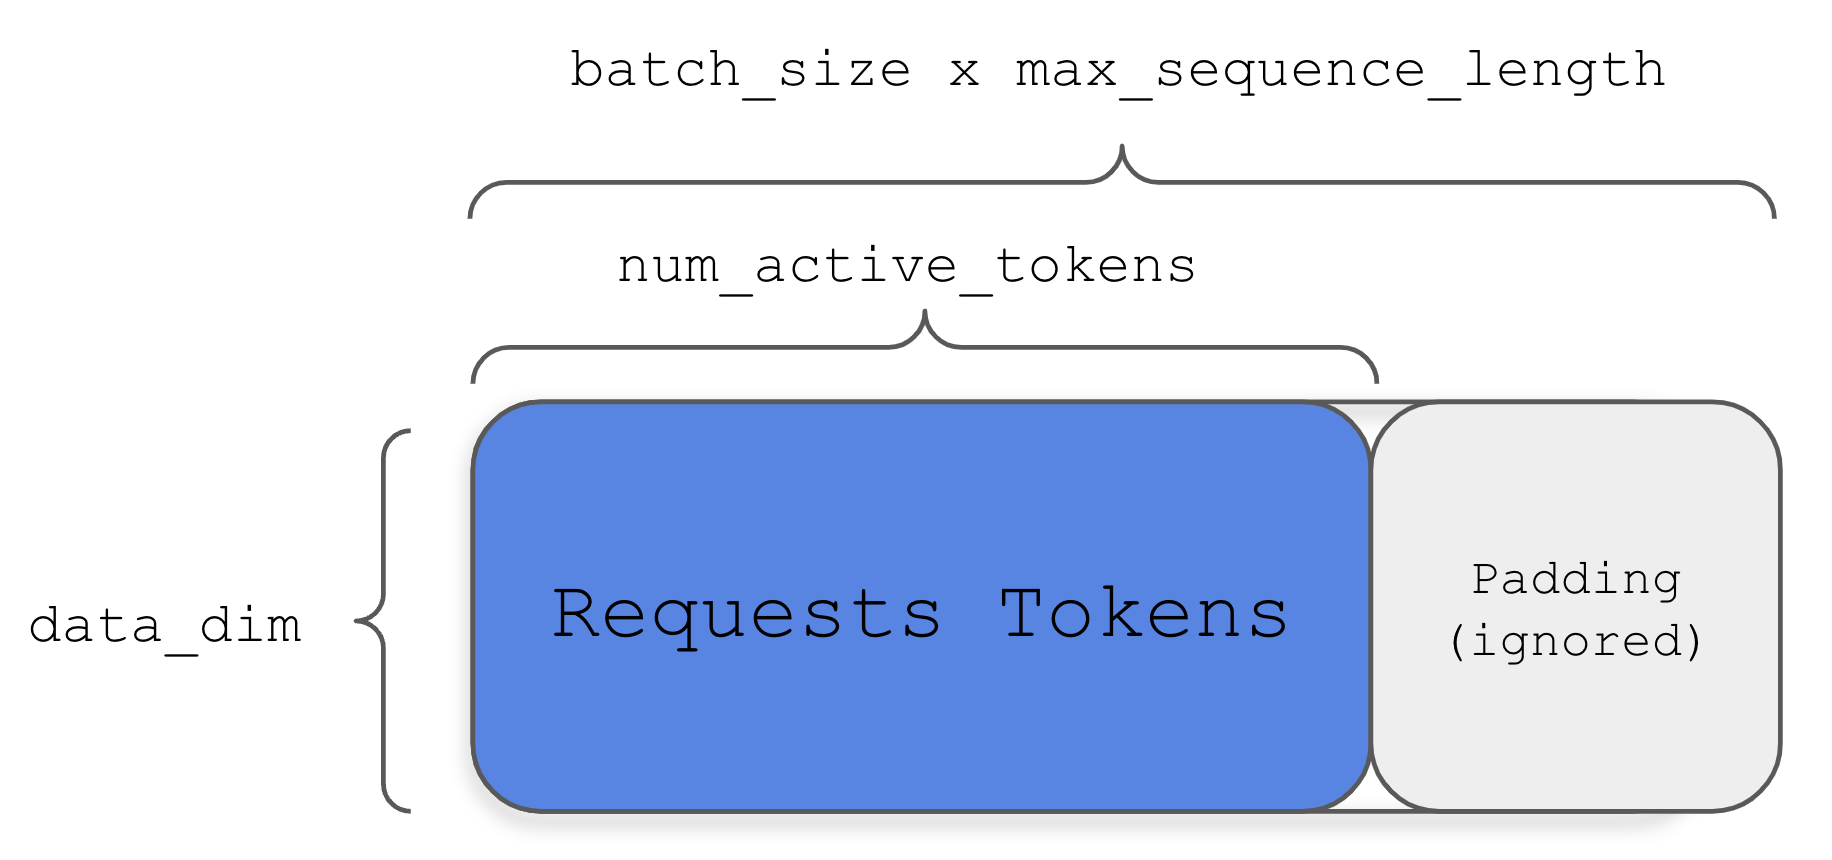
\includegraphics[width=0.6\linewidth]{figures/input_tensor2.png}
    \caption{\textbf{The data layout of the input tensor in the Multi-Head Attention layer}}
    \label{fig:mha-input}
\end{figure}

The second input to the attention kernel is the tensor containing the weights (Figure \ref{fig:mha-weights}). The tensor contains a block of weights for each head, and each block, in turns, contains the the Query, Key, Value and Output projection weights. The first three are used to produce the Query, Key, and Values from the input tokens, whereas the last one is used to generate the final output given all the attention heads.

\begin{figure}[H]
    \centering
    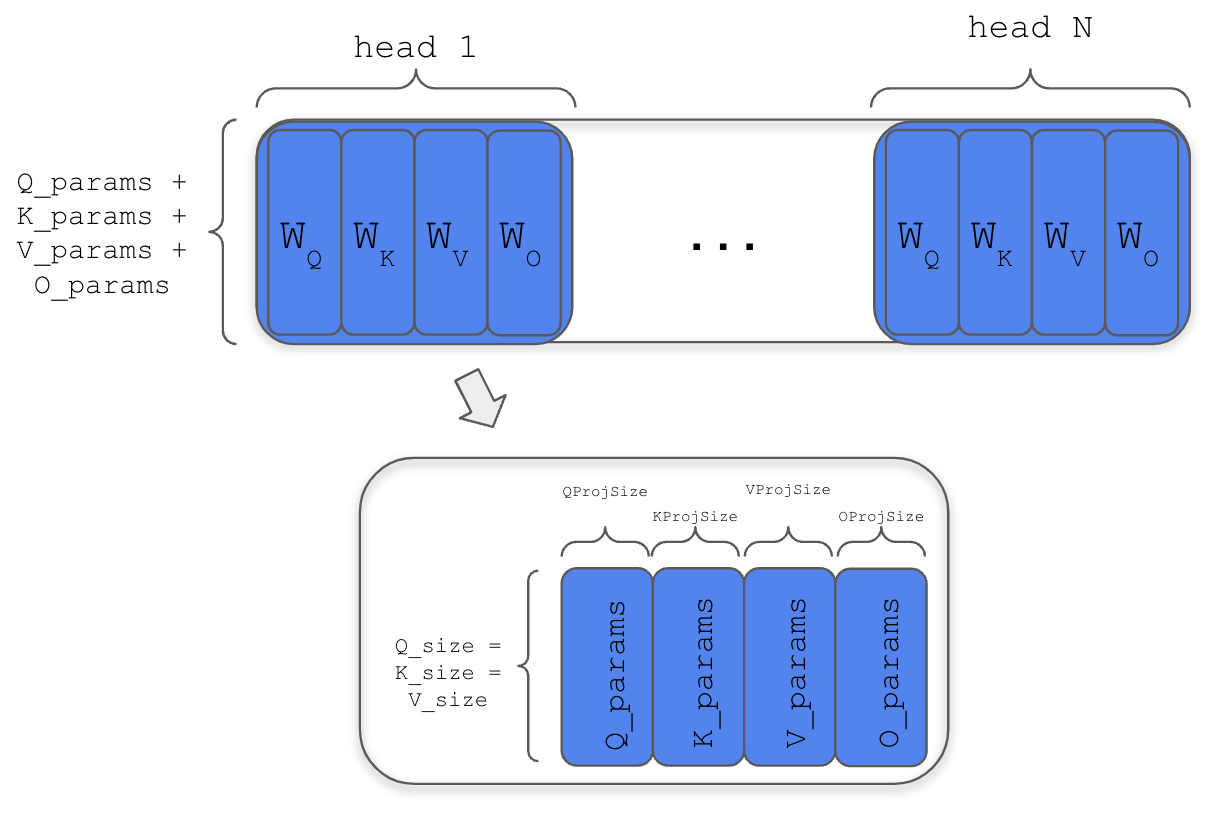
\includegraphics[width=\linewidth]{figures/weights2.png}
    \caption{\textbf{The data layout of the weights tensor in the Multi-Head Attention layer}}
    \label{fig:mha-weights}
\end{figure}

As the first step of the attention kernel, we generate all the Query, Key, and Values from all the input tokens with a single \texttt{cublasGemmStridedBatchedEx}, where the stride is the size of each block of weights corresponding to a single head. We store the result in the Q/K/V projections tensor (Figure \ref{fig:mha-qkv-projs}).

\begin{figure}[H]
    \centering
    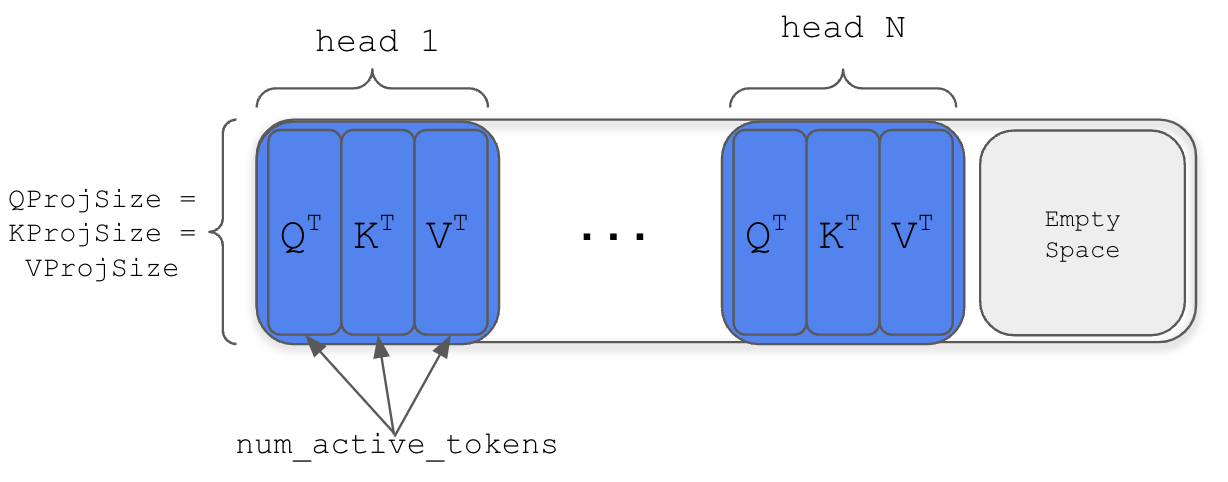
\includegraphics[width=\linewidth]{figures/qkv_proj2.png}
    \caption{\textbf{The data layout of the Q/K/V projections tensor in the Multi-Head Attention layer}}
    \label{fig:mha-qkv-projs}
\end{figure}

Having computed the Q/K/V projections for the current input, we copy the Keys and Values into the cache, so that they can remain accessible across the next iterations. The K-cache (Figure \ref{fig:mha-kcache}) and V-cache (Figure \ref{fig:mha-vcache}) share the same data layout: each tensor is divided into a block for each request, and each such block is further divided into a block for each head. Each head block contains enough room for the Keys or Values for the maximum possible number of tokens in a request.

\begin{figure}[H]
    \centering
    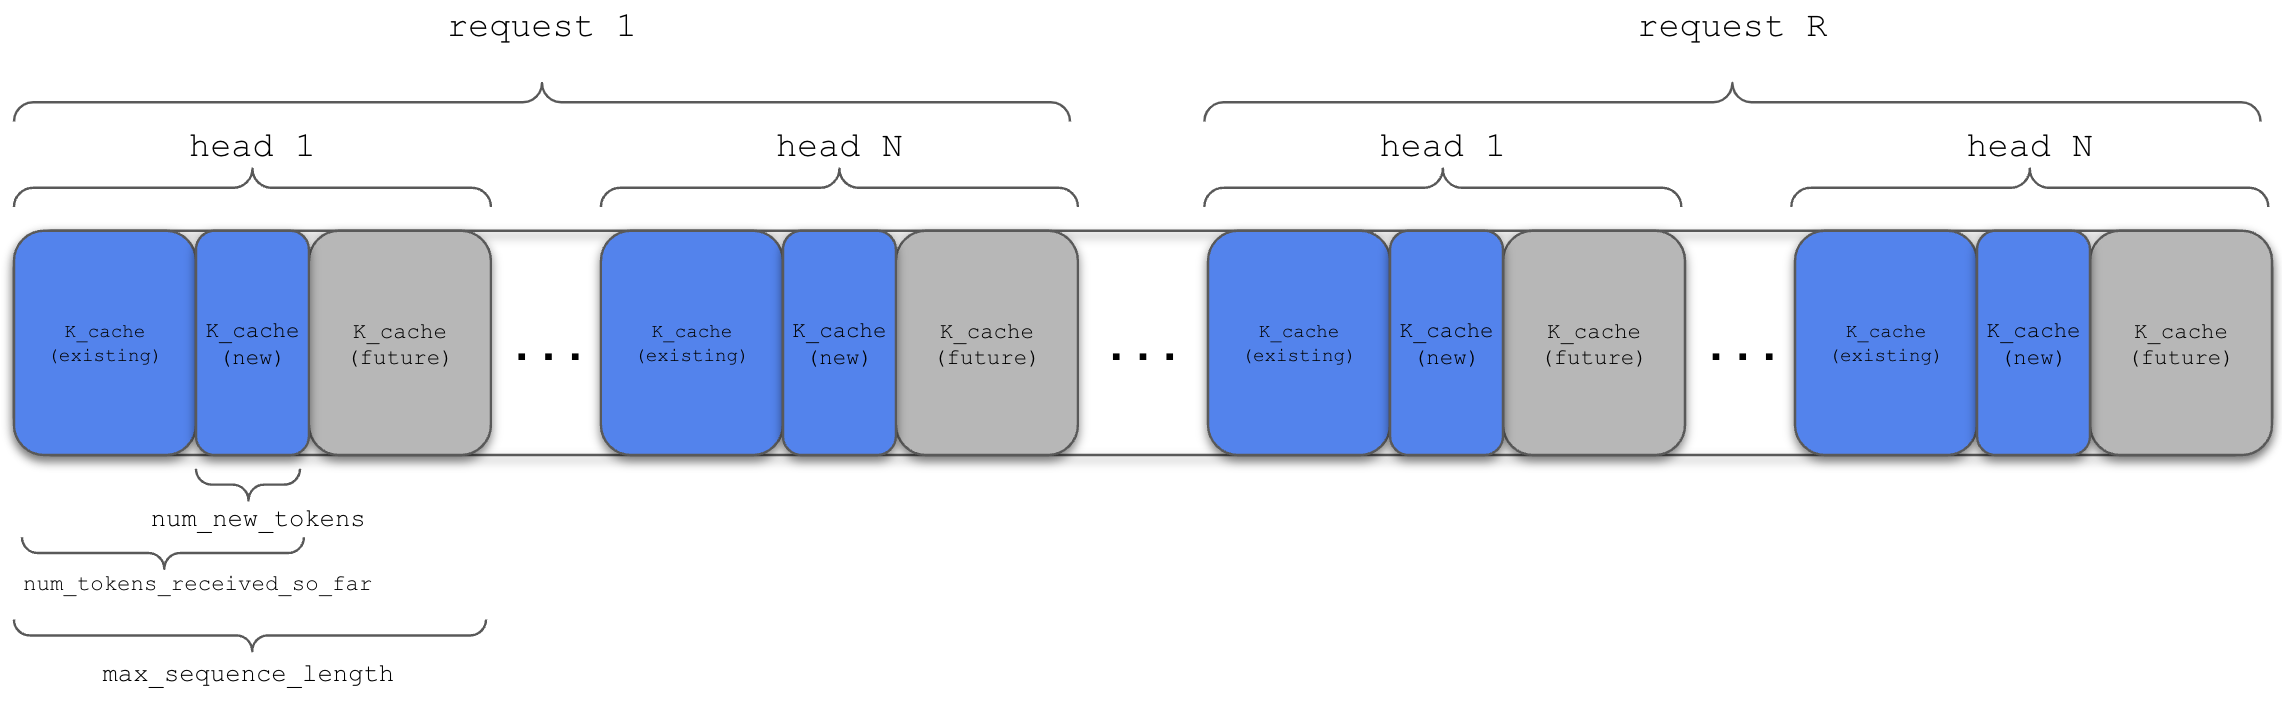
\includegraphics[width=\linewidth]{figures/kcache_tensor2.png}
    \caption{\textbf{The data layout of the K-cache tensor in the Multi-Head Attention layer}}
    \label{fig:mha-kcache}
\end{figure}

\begin{figure}[H]
    \centering
    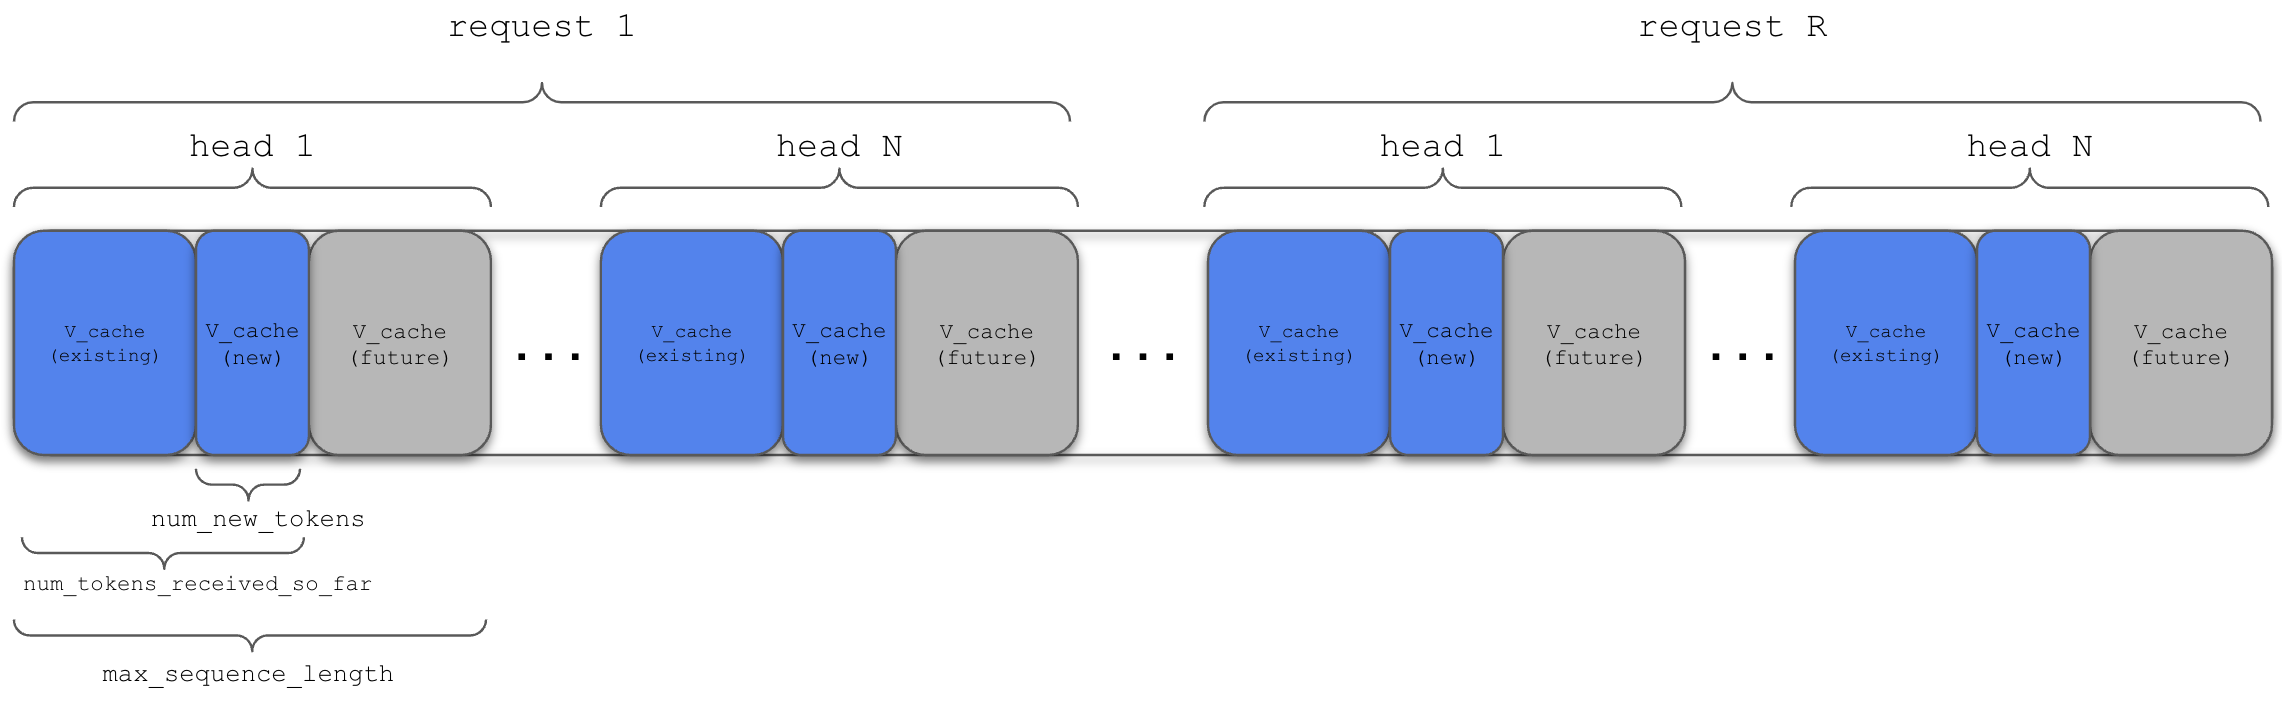
\includegraphics[width=\linewidth]{figures/vcache_tensor2.png}
    \caption{\textbf{The data layout of the V-cache tensor in the Multi-Head Attention layer}}
    \label{fig:mha-vcache}
\end{figure}

After having stored the new Keys and Values in the cache, we proceed to compute the QK products (the product of the Query and Keys for each head), and store them in the QK-product tensor as shown in Figure \ref{fig:mha-qk-products}. In incremental decoding mode, for each request, the Query only contains the projection obtained from the last generated token, whereas the Keys have one entry for each token in the sequence, starting from the beginning. For this reason, each head block in the QK-product tensor has a shape of \texttt{new\_tokens $\times$ num\_tokens\_received\_so\_far}, where \texttt{new\_tokens}$=1$. The next step after generating the QK-products is to compute, for each head block, the softmax with respect to the \texttt{num\_tokens\_received\_so\_far}. Intuitively, the softmax will decide, for each token to be generated, how to weight every other token in the sequence as the token's context. Our operator implements a causal attention, or one when only the preceding tokens are used as a context for generating the next. To implement this, we set all the entries above the diagonal in each head block in the QK-product tensor to $-\infty$. When taking the softmax, these entries will be transformed to $0$, as desired.

\begin{figure}[H]
    \centering
    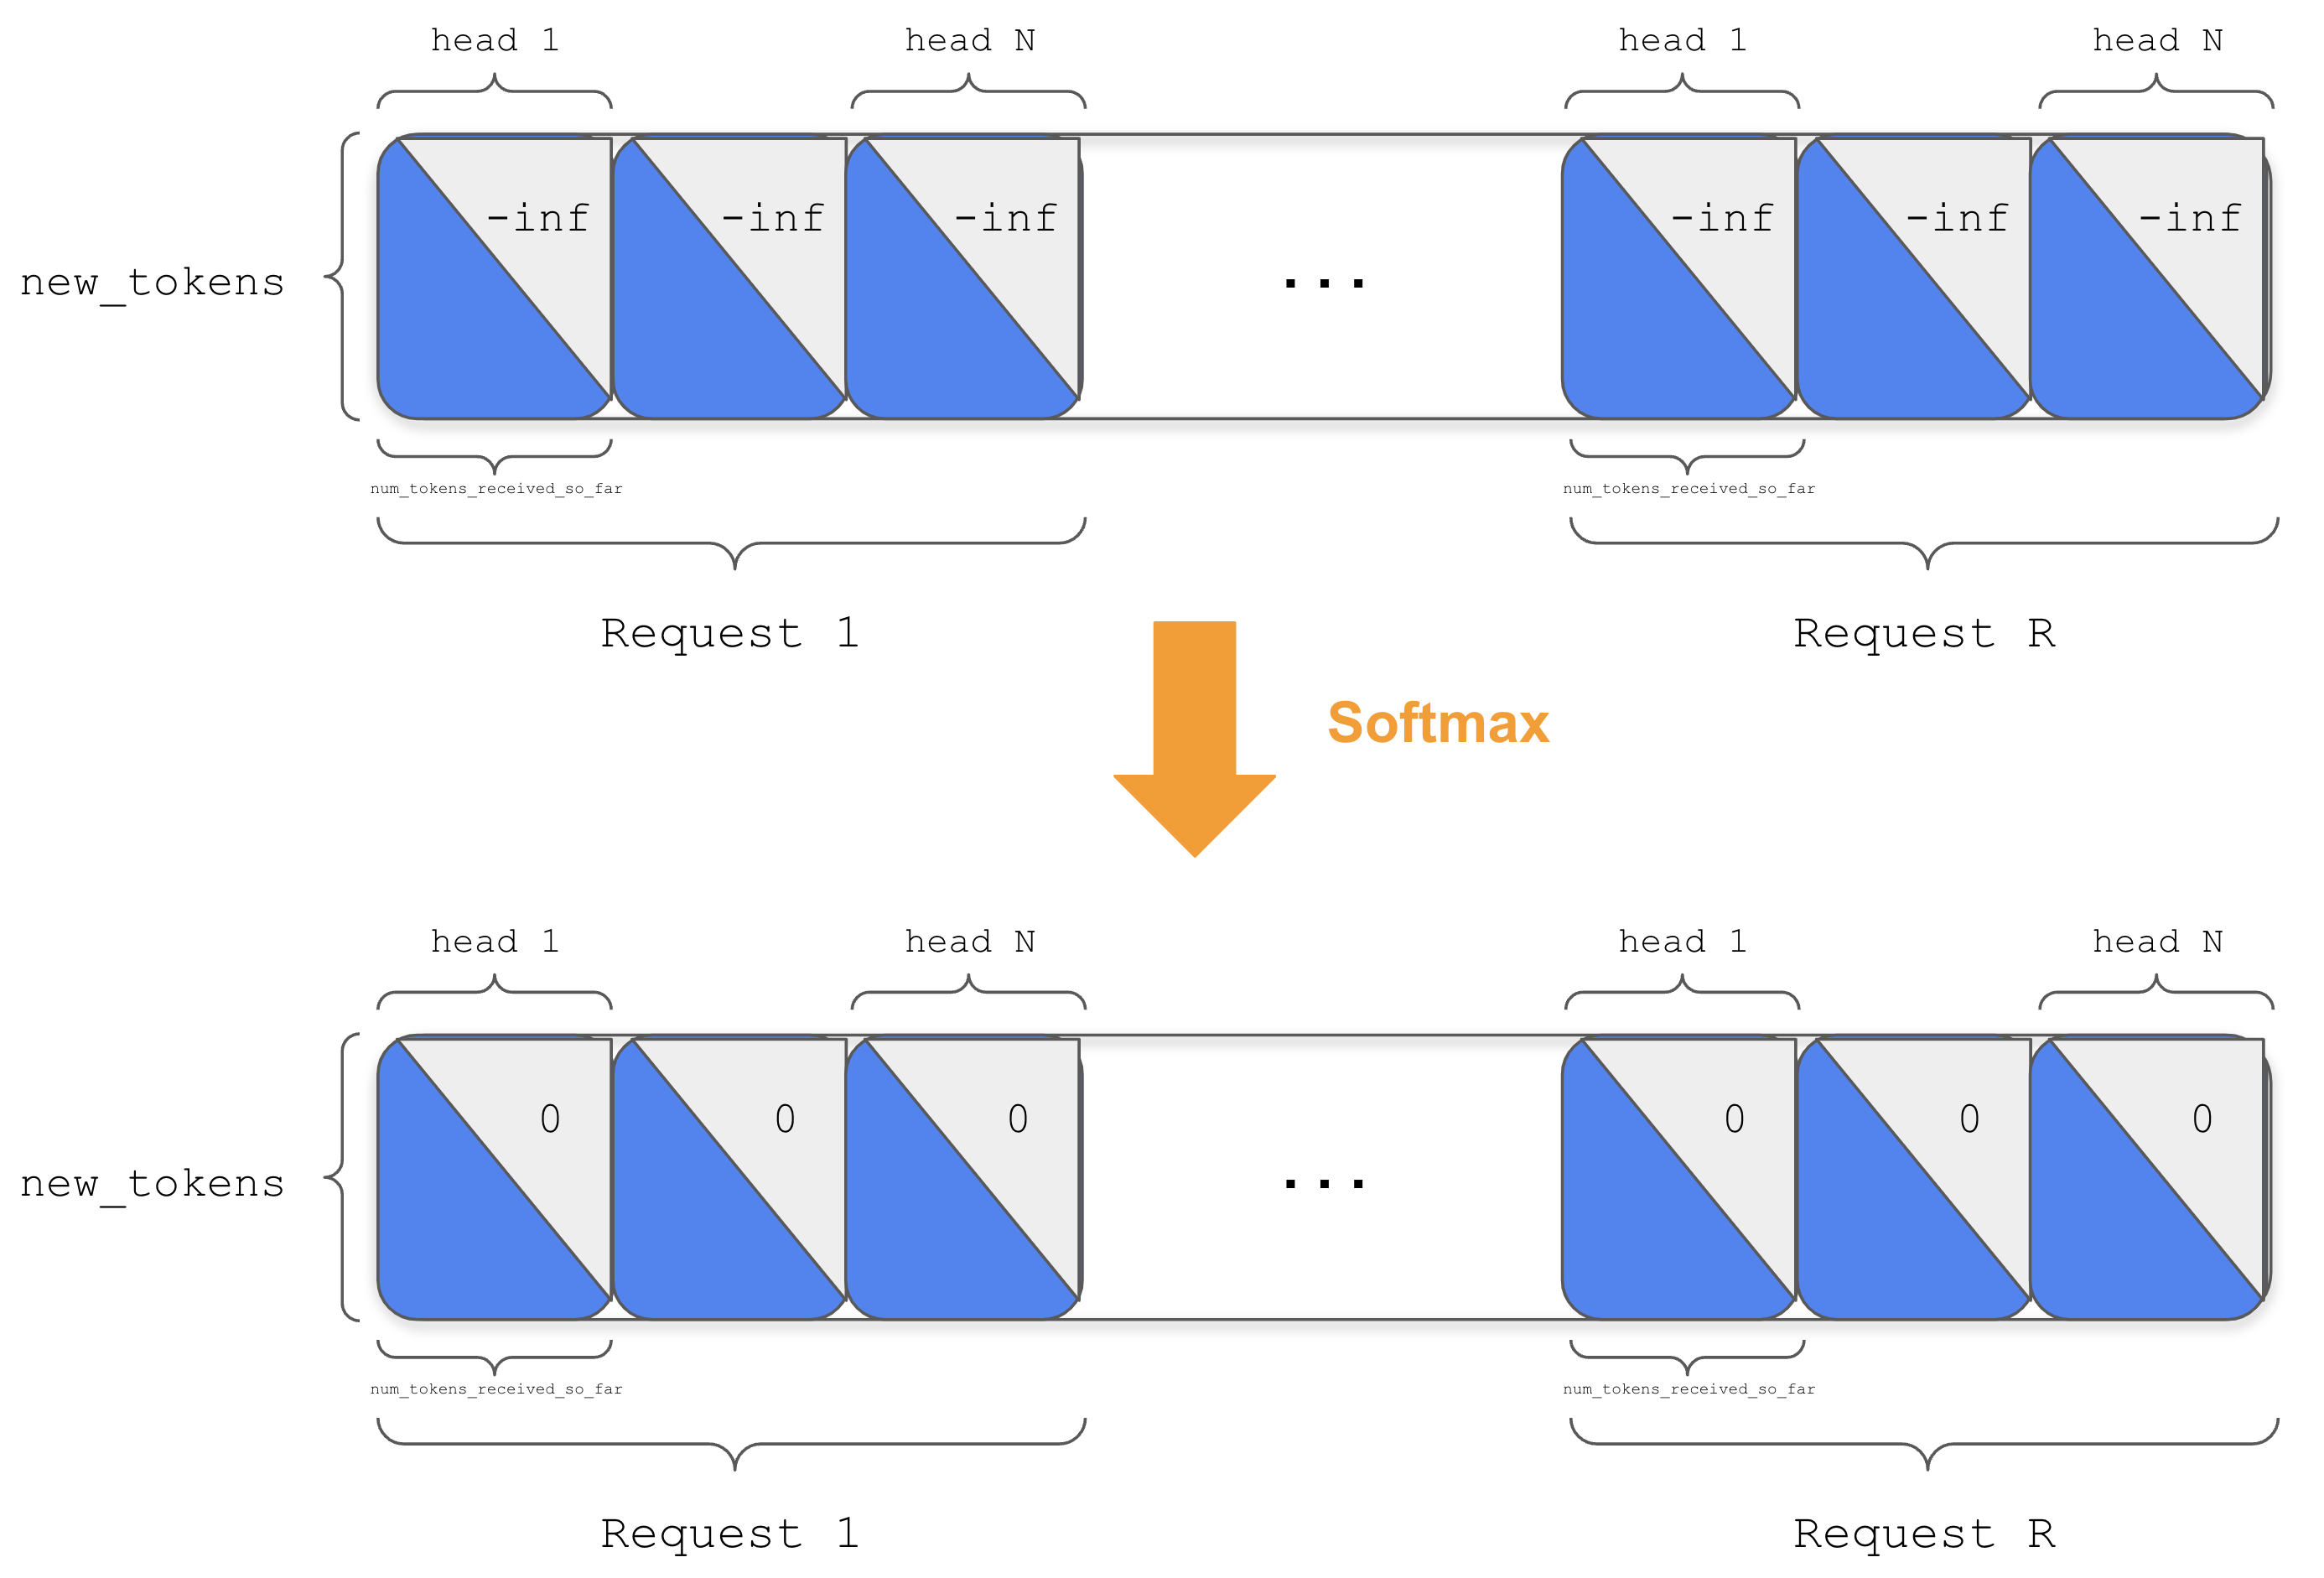
\includegraphics[width=\linewidth]{figures/qk_prods2.png}
    \caption{\textbf{The data layout of the QK-product tensor in the Multi-Head Attention layer}}
    \label{fig:mha-qk-products}
\end{figure}

Next, for each request, we compute the result (Figure \ref{fig:mha-attn-head}) for each attention head by multiplying each head block from the QK-product tensor (after taking the softmax) by the corresponding head block in the V-cache tensor. 

\begin{figure}[H]
    \centering
    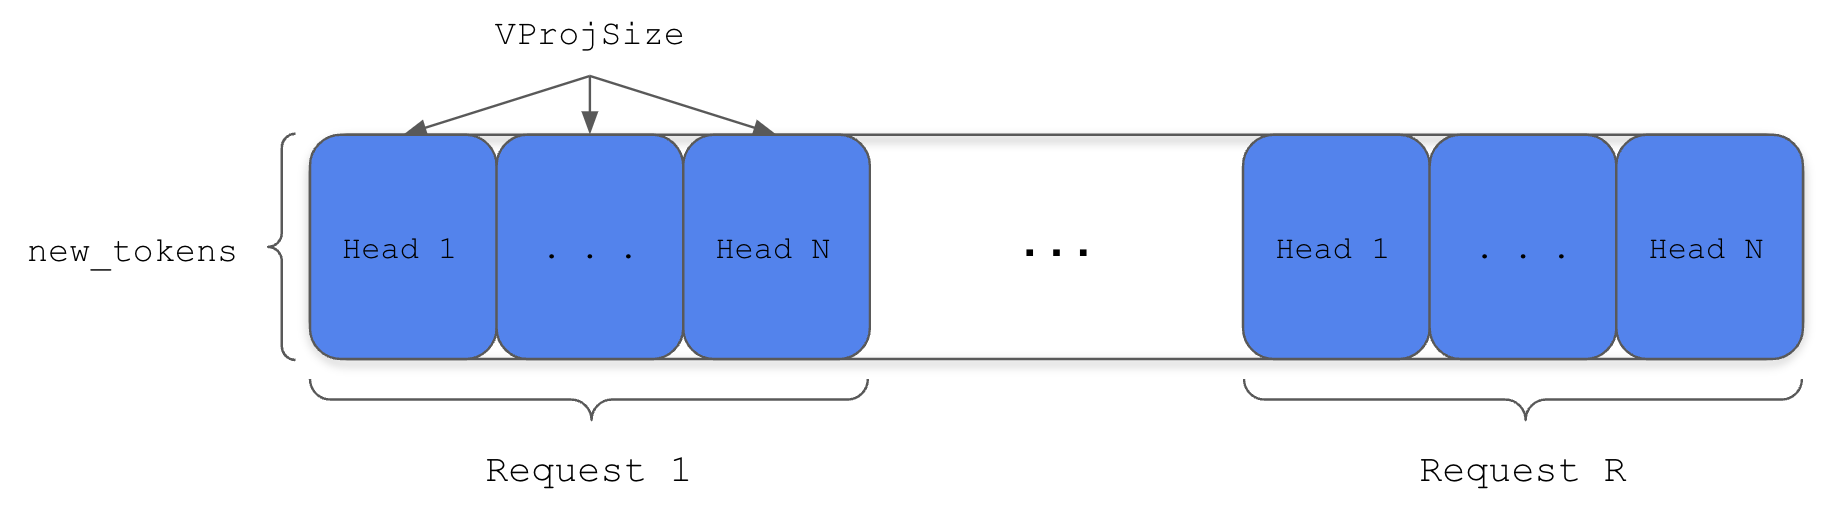
\includegraphics[width=\linewidth]{figures/attn_heads2.png}
    \caption{\textbf{The data layout of the tensor containing the results for each attention head in the Multi-Head Attention layer}}
    \label{fig:mha-attn-head}
\end{figure}

We can now compute the final output, combining the results from all heads, by matrix-multiplying the attention heads tensor (Figure \ref{fig:mha-attn-head}) by the contiguous output projection weight tensor (Figure \ref{fig:w-out}). The latter tensor is so called because it is obtained by combining all the output projection weight slices from the weight tensor (Figure \ref{fig:mha-weights}), so that the slices are contiguous in memory.

\begin{figure}[H]
    \centering
    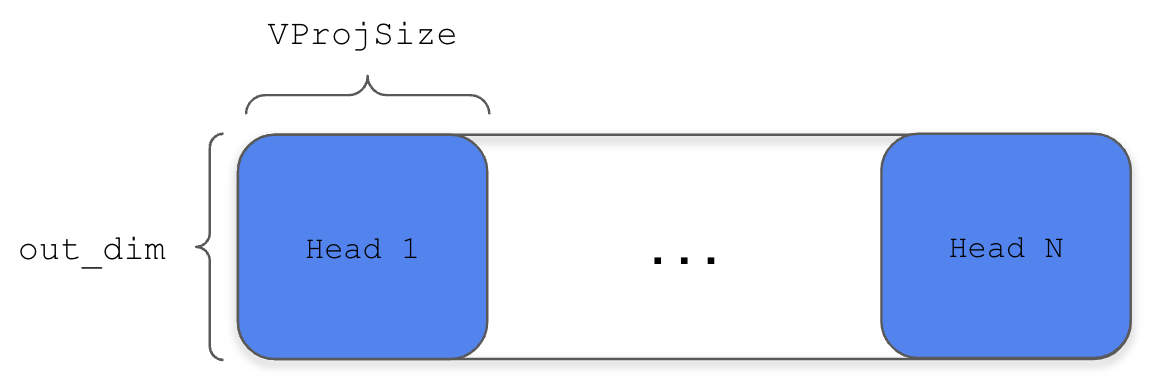
\includegraphics[width=\linewidth]{figures/w_out-contiguous2.png}
    \caption{\textbf{The data layout of the output weights tensor in the Multi-Head Attention layer}}
    \label{fig:w-out}
\end{figure}

\subsection{Optimizations for Speculative Decoding}
Given the \textit{Incremental Multi-Head Attention Kernel} that we described in the section above, we now discuss the changes and optimizations we employed to efficiently support speculative inference. Speculative inference has two stages: first, each speculator generates a sequence of tokens in autoregressive mode; next, we merge the sequences in a single tree and use the large language model to verify which tokens are correct. Each speculator simply runs the multi-head attention in incremental mode, so we can use the kernel from Section \ref{section-simple-mha-kernel} with no additional change. For the verification stage, we describe below how we designed a variant of the \textit{Incremental Multi-Head Attention Kernel} to efficiently support the token tree verification.

In the process of verifying multiple tokens in parallel for each request, we face a challenge: the sequences produced by the speculators may require storing conflicting Key and Value projections in the cache. The simplest solution to overcome this issue is to have separate Key/Value cache tensors for each speculator, as shown in the \textit{Sequence-based Decoding} box in Figure \ref{fig:spec-infer-attention-layout}. This approach allows us to verify each sequence in parallel, but it has a large memory overhead, and computations are often replicated, since the sequences produced by the speculators can often share a prefix. 

An alternative approach is shown in the \textit{Token-based Decoding} box in Figure \ref{fig:spec-infer-attention-layout}. With this approach, we can have a single Key/Value cache tensor, greatly reducing the memory overhead. To avoid conflicts between different sequences, we process one token at a time, placing the result in the slot corresponding to the potential token's depth in the sequence, starting from the beginning of the prompt. By flattening the token tree in DFS order, we can guarantee that, at the time we are processing each branch, the slots to the left of the first token in the branch will not have been overwritten with invalid values for the current branch. The main disadvantage of this approach is that it will be slower, as we won't be able to process multiple tokens in parallel.

Our optimized solution is shown in the \textit{Tree-based Decoding} box in Figure \ref{fig:spec-infer-attention-layout}. Our approach consists of batching together the tokens in the tree such that each token is the subsequent token's parent. This approach will allow us to maximize parallelism while avoiding conflicts.

\begin{figure}[H]
    \centering
    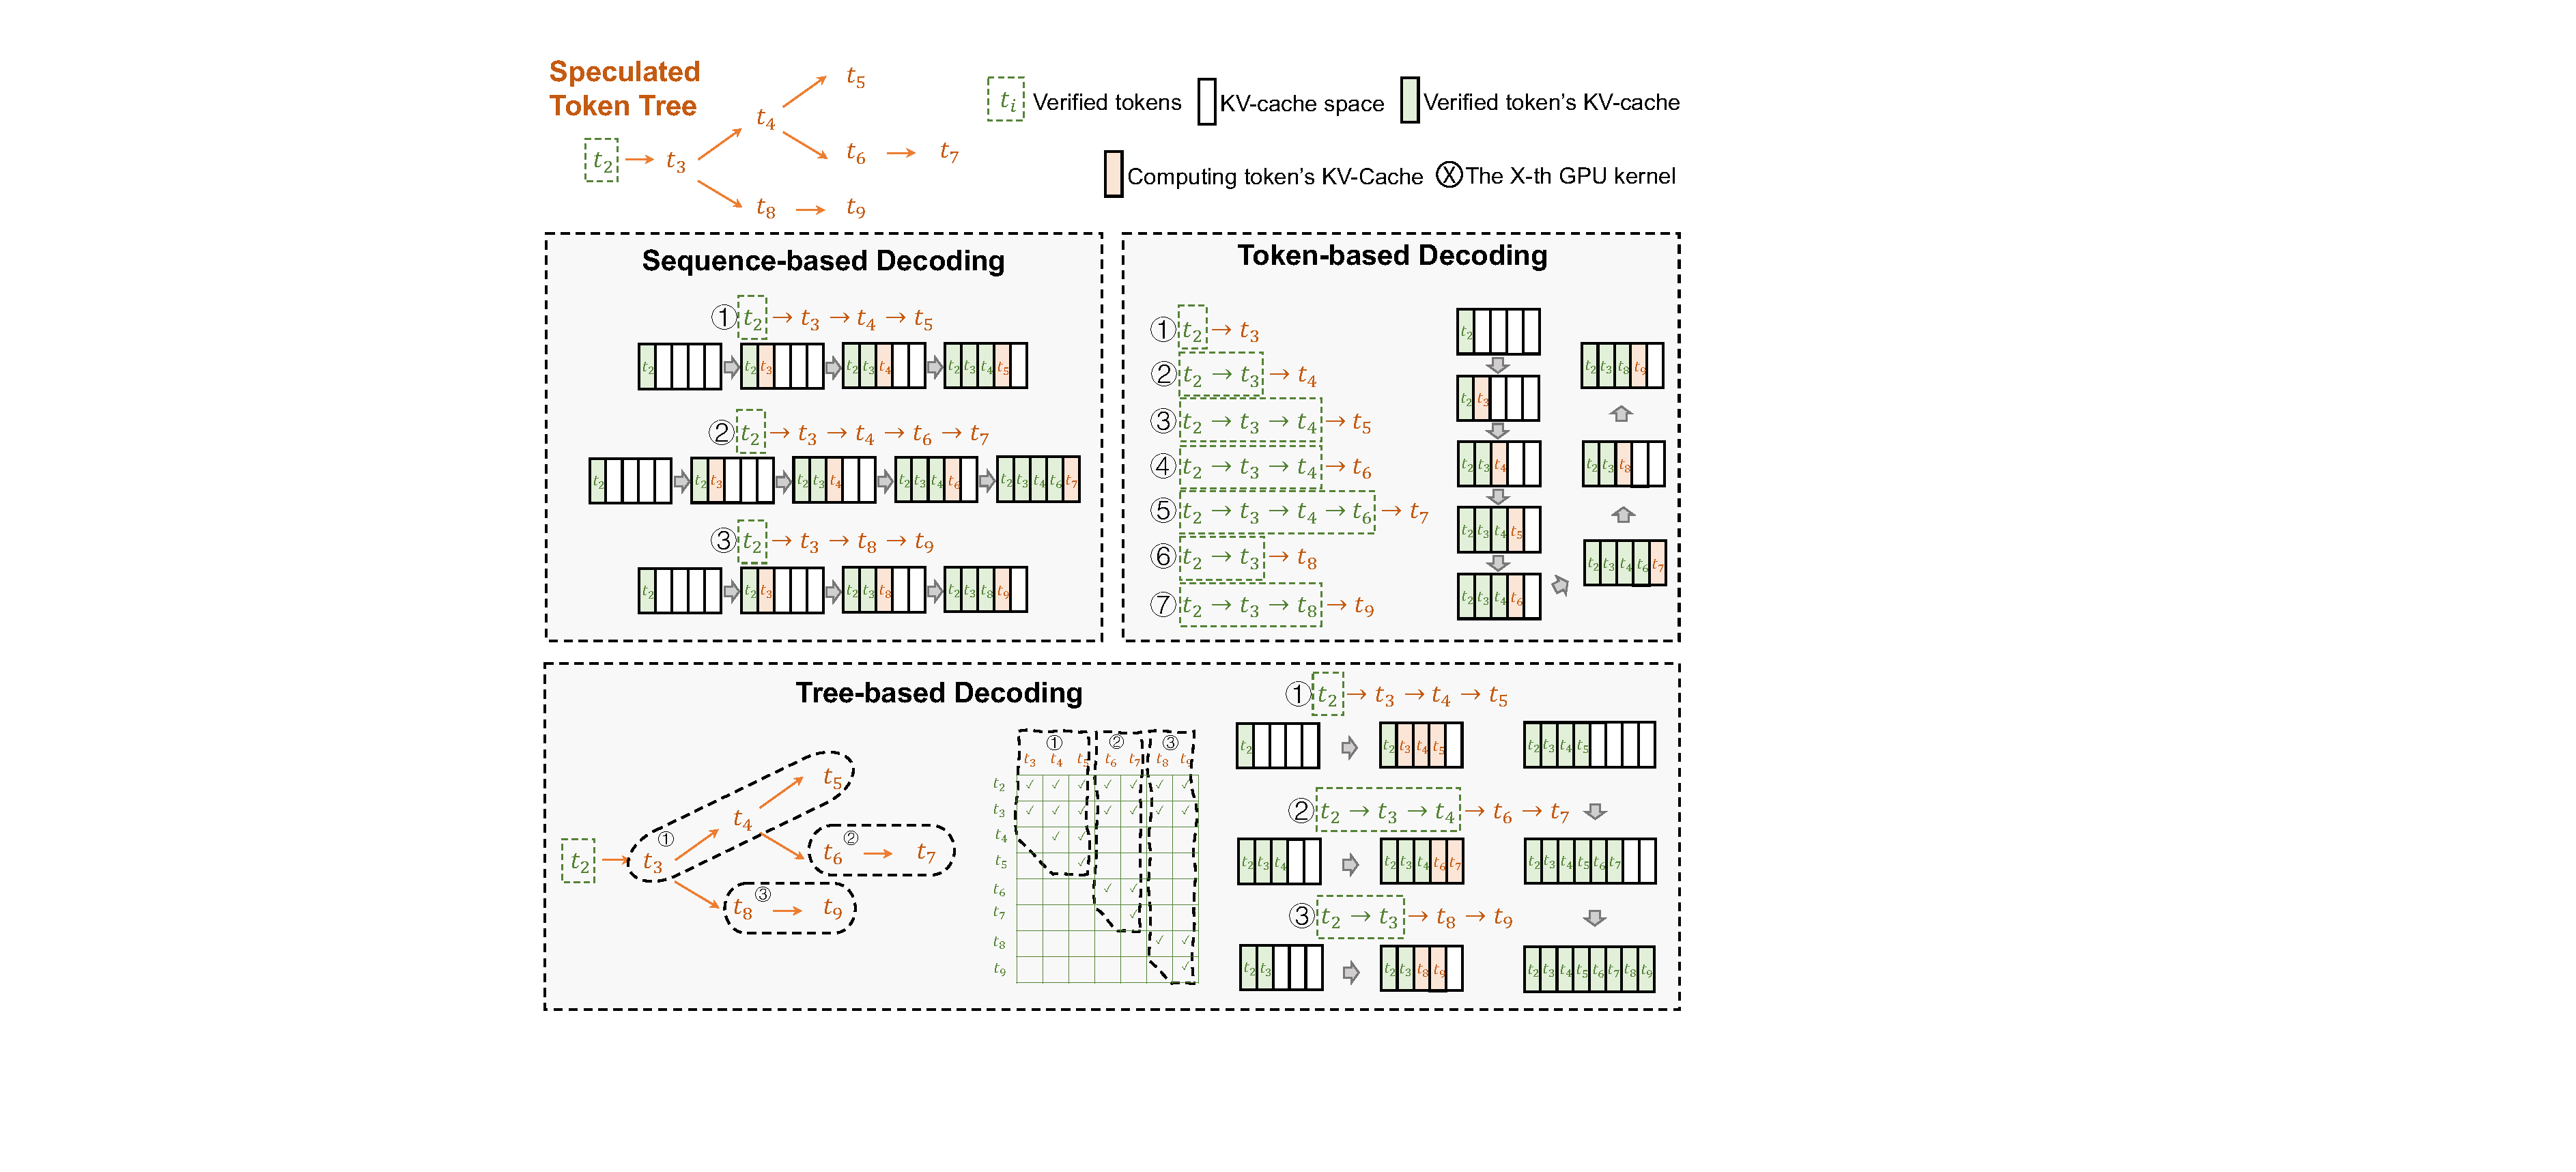
\includegraphics[width=\linewidth]{figures/kv_cache_new4.pdf}
    \caption{\textbf{Naive and optimized solutions to support speculative decoding in ExpertFlow's Multi-Head Attention Kernel}}
    \label{fig:spec-infer-attention-layout}
\end{figure}

\section{Conclusion}
In this chapter, we have discussed the ExpertFlow optimizations at the kernel level. In particular, our system uses two custom CUDA kernels: one to implement the fused-experts operator (Section \ref{section-fused-experts}) and one to implement the multi-head attention (Section \ref{section-simple-mha-kernel}), with a special variant to support token tree verification in the speculative inference scenario.